\chapter{Background}

This section will explain the technical fundamentals which are necessary to understand the full bachelor thesis.

\section{The Scapy program}
\label{sec:scapy}

%UDS stack
\begin{wrapfigure}{r}{0.15\textwidth}
    %
\includegraphics[width=0.1\textwidth]{scapy_logo}
    \raisebox{0pt}[\dimexpr\height-1.5\baselineskip\relax]{
\includegraphics[width=0.15\textwidth]{scapy_logo}}
    %\label{fig:scapy-logo}
\end{wrapfigure}

The homepage of Scapy introduces itself with \cite{scapy}:
\begin{displayquote}
Scapy is a powerful interactive packet manipulation program. It is able to forge or decode packets of a wide number of protocols, send them on the wire, capture them, match requests and replies, and much more.
\end{displayquote}

So, it fulfills the requirements of protocol scanners:
\begin{itemize}
    \item Receive and transmit packets
    \item Support for many physical layers and transport protocols
    \item Simple definition of packet structures
    \item Matching requests with their responses
\end{itemize} 

It is used through a text-based user interface. This has the advantage of being lightweight, and working via ssh connections out-of-the-box. While being mainly a program, it can also be used as a library by importing the necessary classes and interfaces into the own Python program.

It supports Python 3 and also Python 2, even though its support has ended on 1st of January 2020. The following quote from a maintainer explains why \cite{scapy-py2}:

\begin{displayquote}
    Scapy is a tool that can be used in a very large number of situations. Often, you don't get to choose the Python interpreter you have when you run Scapy. So, [...] we need to keep supporting Python 2.7 as long as we can.
\end{displayquote}


\section{The CAN bus}

All communication performed and recorded in this paper with an ECU is done via the Control Area Network bus (CAN).

 Its specification is released in the ISO 11898. Each frame on this bus can transmit up to 8 bytes of payload and has an identifier which a length of either 11- or 29-bits, the former being more common. An identifier does not necessarily have to designate a physical device; it can also indicate one of several software modules of a device.
 The maximum data rate is 1 Mbit/sec with a network length below 40 m. The higher the length, the lower the possible data rate, as can be seen in \autoref{tab:can-speed}.

\begin{table}[htb]
    \centering
    \begin{tabular}{cc}
    \hline
    \textbf{Bus Length (m)} & \textbf{Signaling Rate (Mbps)}\\
    \hline
    40 & 1 \\
    100 & 0.5 \\
    200 & 0.25 \\
    500 & 0.10 \\
    1000 & 0.05 \\
    \hline
\end{tabular}
\caption{Suggested cable lengths for signaling rates of the CAN bus \cite{slla270}.}
\label{tab:can-speed}
\end{table}

\subsection{Advantages for the automotive domain}

This bus is robust because it uses two lines of differential signals for communication. This means that if one wire is driven high, the other one is driven low. Thus, the receiver can reliably detect interferences by comparing these signals.

Moreover, CAN busses are using the bus network topology (see \autoref{fig:with-without-can}). This results in a smaller number of wires compared to star topologies, resulting in lower weight, which is an important factor for manufacturers.

%with-without-can
\begin{figure}[htb]
    \centering
    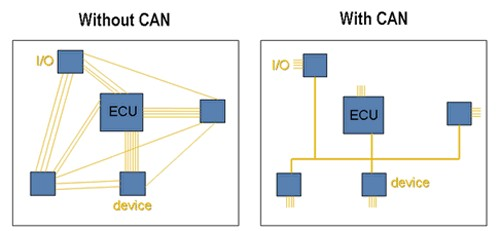
\includegraphics[width=0.7\textwidth]{with-without-can}
    \caption{CAN effect on decreasing the wire quantity \cite{Sharma2016}.}
    \label{fig:with-without-can}
\end{figure}

Last but not least, an important feature for the automotive application domain is the priority support. The lower the identifier, the higher the priority. Hence, if two ECUs transmit a CAN frame at exactly the same time, the frame with the lower identifier wins, the other one is discarded and will be retransmitted. This is called the Carrier Sense Multiple Access with Collision Detection (CSMA/CD) protocol \cite{Sharma2016}. For this reason, diagnostic CAN identifiers tend to have a high identifier \cite{Herrewegen2018}.

\subsection{Security vulnerabilities}

Thinking this one step further, CAN is vulnerable to denial of service attacks. This attack can be performed by flooding the CAN bus with zero-identifier messages resulting in drops of legitimate frames \cite{Buttigieg2017}.

Furthermore, Buttigieg et al. \cite{Buttigieg2017} describe three more security issues of the CAN bus protocol in their paper \emph{Security Issues in Controller Area Networks in Automobiles}.
First, CAN frames do not contain any authentication information. An ECU receiving a message is not able to distinguish between a message from a legitimate ECU and a malicious one \cite{Buttigieg2017}. So, for example, if the state of an ECU is changed to a higher privileged state, all devices, including malicious ones, will have access to its newly unlocked services and information. Countermeasures exist in the form of performing authentication, but there is no satisfying solution yet, which fulfills cost-effectiveness, backward compatibility, support for vehicle repair and maintenance, sufficient implementation details, and acceptable overhead \cite{Bozdal2020}.
Also, originally, CAN bus networks lacked network segmentation, since each message is broadcasted and received by each node of the network \cite{Buttigieg2017}. Nowadays, car networks are usually divided into less and more critical segments by so-called Gateway ECUs \cite{Bozdal2020}. Despite the increase in the level of security, this makes it more difficult to maintain the system, which is associated with increased costs \cite{Bozdal2020}.
The final security vulnerability is the lack of data encryption \cite{Buttigieg2017}. Lightweight encryption systems could be implemented, but are limited by the short length of the data field (8 bytes) and the limited computing power of ECUs \cite{Bozdal2020}.

Since all countermeasures described in the previous paragraph are limited, Intrusion Detection Systems (IDS) are emerging, with the advantages of not having to change the current CAN controller and not increasing bus traffic \cite{Bozdal2020}. A proof of concept of such systems was implemented by eMundo in preparation for the PetS3 project \cite{spahn2018}.

\subsection{Virtual CAN interfaces and using the can-utils}
\label{subsubsec:can-utils}

Virtual CAN interfaces can be used for simulations or simple tests. They are supported natively by Linux without additional actions.
To create a virtual CAN interface, only one command in a Linux shell is required (see line 1 of \autoref{lst:can-utils}).

\begin{listing}[H]
\begin{minted}
[frame=single,
framerule=0pt,
framesep=2mm,
baselinestretch=1.2,
bgcolor=VeryLightGray,
fontsize=\footnotesize,
linenos]{text}
sudo ip link add vcan0 type vcan
candump vcan0
candump -l vcan0
cansend vcan0 123#01.02
\end{minted}
\caption{How to use the can-utils.}
\label{lst:can-utils}
\end{listing}

The most common toolkit to work with the CAN bus are the can-utils \cite{can-utils}, which can be usually installed with the package manager of the distributions. The candump command (line 2) displays all messages of the CAN bus on interface \mintinline{text}{vcan0} in a terminal:

Adding the \mintinline{text}{-l} option changes the output to be more compact instead of human-readable and stores the received traffic in a \mintinline{text}{candump.log} file (line 3). All traffic recorded in this work was done with this command.

For sake of completeness, the \mintinline{text}{cansend} command (line 4) sends a CAN frame with the identifier 0x123 and the payload \mintinline{text}{0x01 0x02}:

\section{The ISO-TP transport protocol for CAN}

CAN frames have a payload size of 8 bytes. This is sufficient for most UDS requests, but not for many UDS responses. Thus, ISO-TP is used as the transport protocol on the CAN bus for UDS communication.

It is defined in ISO 15765-2 and increases the payload size from 8 bytes to 4095 bytes per message. At least one byte of the data of each CAN frame is then transport protocol information, indicating whether this frame contains the entire application data or only a fragment of it, with more frames to come.

\section{The UDS protocol}

UDS stands for \emph{Unified diagnostic services} and is an application protocol defined in ISO 14229. This protocol defines the structures of request and response data for diagnostic purposes sent over an arbitrary data link \cite{iso14229}.

The reason for the development of such a protocol was that the cars developed in the last decades were more and more able to diagnose themselves. A car repair shop only had to request this information from the car. But since there was no universal standard, car manufacturers tended to implement company-specific protocols for this purpose. UDS solves this by being an international standard and not company-specific. The \emph{Unified} in its name underlines this. 

%UDS stack
\begin{figure}[htb]
    \centering
    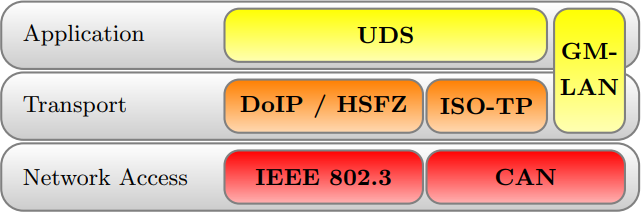
\includegraphics[width=0.7\textwidth]{uds-stack}
    \caption{The most common protocol stack for UDS \cite{Weiss2020}.}
    \label{fig:uds-stack}
\end{figure}

As shown in \autoref{fig:uds-stack}, the most common data links for the UDS protocol are the Ethernet and the CAN bus. Others can and are used as well, explicitly stated in the UDS standard are FlexRay, K-Line and LIN.

\subsection{Data structure}

\begin{figure}[htb]
    \centering
    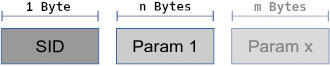
\includegraphics[width=0.5\textwidth]{uds-structure}
    \caption{The structure of UDS requests.}
    \label{fig:uds-structure}
\end{figure}

\autoref{fig:uds-structure} shows how UDS requests are structured. Each service is identified by a Service Identifier (SID). This identifier is the first byte in all UDS data. It must not be confused with the identifier of the CAN frame. Then at least one parameter follows. Most common is only one parameter, but services with multiple parameters exist too.
Negative responses have the SID 0x7f.
For positive responses it is defined as 0x40 added to the SID. Thus, a request with SID 0x27 would be responded with 0x27 + 0x40 = 0x67 (see \autoref{fig:key-seed}).

\subsection{Services}
\label{subsubsec:uds-services}

UDS defines various services with different purposes. The ones used later in this paper are explained here.

The Routine Control (RC) service allows managing predefined routines on the ECU. They can be started, stopped or their results requested. It has two parameters, namely the desired action and the identifier of the routine.

Another service is called Read Data By Identifier (RDBI). With this service, it is possible to retrieve one or more values of an ECU. This can be static information like the software version or dynamic values such as the current readings of sensors. The structure of RDBI requests is simple as it only contains an identifier as parameter.

The Diagnostic Session Control (DSC) service is used to enable different diagnostic states in the ECU, and the Security Access (SA) service to unlock restricted access to data or services. They are explained in more detail in the next section, as they affect the state of ECUs.

\subsection{States}
\label{subsec:states}

There is always exactly one global UDS state active for an ECU. It influences the behavior of the ECU and can be changed by sending specific requests. Just a few services are able to accomplish this. For example, sending a request to the SA or DSC service of an ECU may affect its state. Whether the ECU has actually changed the state can be easily determined by checking whether the sender received a positive or negative response from the ECU.

\begin{figure}[htb]
    \centering
    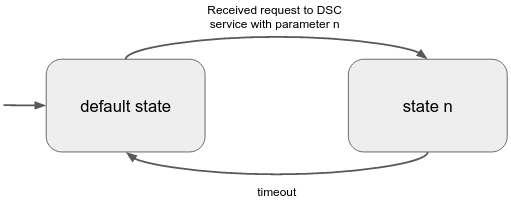
\includegraphics[width=0.7\textwidth]{ecu-state-behavior}
    \caption{State machine example of ECUs for UDS with the DSC service.}
    \label{fig:ecu-state-behavior}
\end{figure}

The default state is the active state after the ECU is switched on. Without an external request, it remains in this state. \autoref{fig:ecu-state-behavior} illustrates the behavior of the ECU when a request is received for the DSC service and parameter value $n$. In the DSC service, each parameter value specifies a state. Thus, if the ECU designers integrated a state for $n$, the controller will respond positively. It will now remain in this state until there has been no UDS communication for usually five seconds, then it will automatically return to the default state. If the ECU designers did not integrate such a state, it will answer with a negative response and remain in its current state.

The Security Access service uses the challenge–response authentication, in automotive terminology called seed-key protocol. The ECU sends a randomly generated value (the seed) to the client. Both devices generate a response (the key) based on the seed and the client sends its response to the ECU. If the keys match for the received and the generated response for the ECU, the client is authenticated \cite{iso14229}.

\begin{figure}[htb]
    \centering
    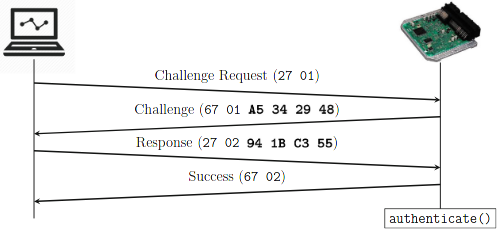
\includegraphics[width=0.7\textwidth]{key-seed}
    \caption{The challenge-response protocol \cite{Herrewegen2018}.}
    \label{fig:key-seed}
\end{figure}


\section{The UDS Scanner}

The UDS Scanner was implemented in Scapy for the PetS3 project.

\subsection{Purpose}

\begin{figure}[htb]
    \centering
    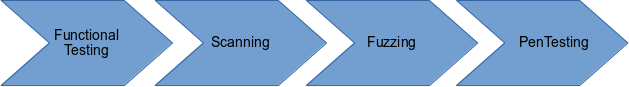
\includegraphics[width=0.8\textwidth]{automotive-security-testing-process}
    \caption{The Automotive Security Testing process.}
    \label{fig:automotive-security-testing-process}
\end{figure}

As \autoref{fig:automotive-security-testing-process} shows, the security testing process in the automotive domain contains a scanning step that aims to detect what services of a protocol are implemented and what information can be retrieved there \cite{Bayer2015}. The UDS Scanner fulfills these tasks. It can also be used for fuzzing, even though scanning is its main use-case. The retrieved information answers the following questions:

\begin{itemize}
\item Which services are supported?
\item What information can be read with these services?
\item What control options does the ECU offer?
\item Which states does it have and how does it behave in each case?
\end{itemize}


\subsection{Procedure}

The UDS Scanner starts with scanning each service for the default state of the ECU (see \autoref{subsec:states}). While doing so, it detects new states, which will be scanned subsequently. So as long as new states are found during an iteration, the scan continues. After each iteration, the ECU is reset to return to the default state. Then, the next state to be scanned is activated by sending a sequence of UDS requests, which is an edge of the UDS Scanner's internally built state machine. An ECU reset is usually done by switching off the ECU, waiting a few seconds, and switching it on again, although there is an ECU Reset service in the UDS protocol. However, its specification states that the behavior is implementation-specific, so a power-based reset is the cleaner way.

\autoref{lst:uds-scanner} aims to make the procedure easier to understand:

\begin{listing}[H]
\begin{minted}
[frame=single,
framerule=0pt,
framesep=2mm,
baselinestretch=1.2,
bgcolor=VeryLightGray,
fontsize=\footnotesize,
linenos]
{python}
class UDS_Scanner:
    def scan():
       states = [default_state]
       for state in states:
           ecu.reset()
           ecu.enter_state(state)
           for service in service_list:
               service.scan() # detects new states
       ecu.reset()
\end{minted}
\caption{Procedure of the UDS Scanner.}
\label{lst:uds-scanner}
\end{listing}
